\documentclass[12pt]{article}
\usepackage[utf8]{inputenc}
\usepackage[letterpaper, margin=1in]{geometry}
\usepackage{graphicx}
\usepackage{mathptmx}
\usepackage{float}
\usepackage[cmex10]{amsmath}
\usepackage{amsthm,amssymb}
\usepackage{url}
\urlstyle{same} 
\def\UrlBreaks{\do\/\do-}
\usepackage{breakurl}
\usepackage{fancybox}
\usepackage{breqn}
\usepackage{array}
\usepackage{caption}
\usepackage{subcaption}
\usepackage{comment}
\usepackage[english]{babel}
\usepackage[acronym,nomain]{glossaries} % list of acronyms
\usepackage{xurl}
\usepackage{cite} % math and engineering style citations
\usepackage{multicol}
\usepackage{multirow}
\usepackage{mathptmx}
\usepackage{float}
\usepackage{lipsum}
\usepackage{framed}
\usepackage[T1]{fontenc}
\usepackage[pdfpagelabels,pdfusetitle,colorlinks=false,pdfborder={0 0 0}]{hyperref}

\renewcommand{\arraystretch}{1.2}

\sloppy

\newcolumntype{C}[1]{>{\centering\let\newline\\\arraybackslash\hspace{0pt}}m{#1-2\tabcolsep}}

\title{DC Optimal Dispatch Modeling of a Distribution Level Power Grid with Static and Vehicle-to-Grid (V2G) Energy Storage}
\author{Aaron I. Rabinowitz}
\date{}

\newacronym{ghg}{GHG}{Green-House Gas}
\newacronym{fe}{FE}{Fuel Economy}
\newacronym{ee}{EE}{Energy Economy}
\newacronym{epa}{EPA}{Environmental Protection Agency}
\newacronym{oem}{OEM}{Original Equipment Manufacturer}
\newacronym{ice}{ICE}{Internal Combustion Engine}
\newacronym{icv}{ICV}{Internal Combustion Vehicle}
\newacronym{icev}{ICEV}{Internal Combustion Engine Vehicle}
\newacronym{em}{EM}{Electric Motor}
\newacronym{hev}{HEV}{Hybrid Electric Vehicle}
\newacronym{ev}{EV}{Electric Vehicle}
\newacronym{phev}{PHEV}{Plug-in Hybrid Electric Vehicle}
\newacronym{lrphev}{LR-PHEV}{Long Range PHEV}
\newacronym{srphev}{SR-PHEV}{Short Range PHEV}
\newacronym{mhev}{MHEV}{Mild Hybrid Electric Vehicle}
\newacronym{pev}{PEV}{Plug-in Electric Vehicle}
\newacronym{bev}{BEV}{Battery Electric Vehicle}
\newacronym{cbev}{CBEV}{City BEV}
\newacronym{afv}{AFV}{Alternative Fuel Vehicle}
\newacronym{fcev}{FCEV}{Fuel Cell Electric Vehicle}
\newacronym{cav}{CAV}{Connected Autonomous Vehicle}
\newacronym{fc}{FC}{Fuel Consumption}
\newacronym{ec}{EC}{Energy Consumption}
\newacronym{dtto}{DTTO}{Discrete Time Trajectory Optimization}
\newacronym{udto}{UDTO}{Uniformly Discretized Trajectory Optimization}
\newacronym{sto}{STO}{Spline Trajectory Optimization}
\newacronym{rbed}{RBED}{Rules-Based Eco-Driving}
\newacronym{cidm}{CIDM}{Cooperative Intelligent Driver Model}
\newacronym{idm}{IDM}{Intelligent Driver Model}
\newacronym{soc}{SOC}{State of Charge}
\newacronym{ocp}{OCP}{Optimal Control Problem}
\newacronym{ttc}{TTC}{Time-To-Collision}
\newacronym{dp}{DP}{Dynamic Programming}
\newacronym{ga}{GA}{Genetic Algorithm}
\newacronym{sdm}{SDM}{Smart Driver Model}
\newacronym{v2i}{V2I}{Vehicle to Infrastructure}
\newacronym{v2v}{V2V}{Vehicle to Vehicle}
\newacronym{v2x}{V2X}{Vehicle to Everything}
\newacronym{hil}{HIL}{Hardware In Loop}
\newacronym{pso}{PSO}{Particle Swarm Optimization}
\newacronym{dt}{DT}{Direct Transcription}
\newacronym{oedt}{OEDT}{Optimal Eco-Driving Trace}
\newacronym{fods}{FODS}{Forward Object Detection System}
\newacronym{cas}{CAS}{Collision Aviodance System}
\newacronym{acc}{ACC}{Adaptive Cruise Control}
\newacronym{obu}{OBU}{On-Board Unit}
\newacronym{rsu}{RSU}{Road-Side Unit}
\newacronym{sae}{SAE}{Society of Automotive Engineers}
\newacronym{adas}{ADAS}{Advanced Driver Assistance System}
\newacronym{edc}{EDC}{Eco-Driving Control}
\newacronym{lv}{LV}{Lead Vehicle}
\newacronym{ss}{SS}{Segment Speeds}
\newacronym{hs}{HS}{Historical Speeds}
\newacronym{spat}{SPAT}{Signal Phase and Timing}
\newacronym{map}{MAP}{Positions of Subsequent Traffic Lights}
\newacronym{al2n}{AL2N}{Acceleration L\textsuperscript{2} Norm}
\newacronym{rpc}{RPC}{Road Power Cost}
\newacronym{bpc}{BPC}{Battery Power Cost}
\newacronym{fecc}{FECC}{Fitted Equivalent Consumption Cost}
\newacronym{ipopt}{IPOPT}{Interior-Point Optimization}
\newacronym{dtnlp}{DTNLP}{Discreet-Time Non-Linear Programming}
\newacronym{snlp}{SNLP}{Spline Non-Linear Programming}
\newacronym{sga}{SGA}{Spline Genetic Algorithm}
\newacronym{spso}{SPSO}{Spline Particle Swarm Optimization}
\newacronym{2sdp}{2SDP}{2 State Dynamic Programming}
\newacronym{aos}{AOS}{Approximate Optimal Spline}
\newacronym{pchip}{PCHIP}{Piecewise Cubic Hermitic Interpolation Polynomial}
\newacronym{nrel}{NREL}{National Renewable Energy Laboratory}
\newacronym{fastsim}{FASTSim}{Future Automotive Systems Technology Simulator}
\newacronym{mfei}{MFEI}{Mean Fuel Economy Improvement}
\newacronym{pas}{PAS}{Percent Acceptable Solutions}
\newacronym{mrt}{MRT}{Mean Run-Time}
\newacronym{mpc}{MPC}{Model Predictive Control}
\newacronym{adp}{ADP}{Approximate Dynamic Programming}
\newacronym{rl}{RL}{Reinforcement Learning}
\newacronym{mbrl}{MBRL}{Model Based Reinforcement Learning}
\newacronym{nlp}{NLP}{Non-Linear Programming}
\newacronym{nhtsa}{NHTSA}{National Highway Traffic Safety Administration}
\newacronym{aeb}{AEB}{Automatic Emergency Braking}
\newacronym{tsdc}{TSDC}{Transportation Secure Data Center}
\newacronym{anl}{ANL}{Argonne National Lab}
\newacronym{d3}{D\textsuperscript{3}}{Downloadable Dynamometer Database}
\newacronym{cd}{C\textsubscript{D}}{Coefficient of Drag}
\newacronym{crr}{C\textsubscript{RR}}{Coefficient of Rolling Resistance}
\newacronym{mape}{MAPE}{Mean Absolute Percentage Error}
\newacronym{evse}{EVSE}{Electric Vehicle Support Infrastructure}
\newacronym{ld}{LD}{Light Duty}
\newacronym{md}{MD}{Medium Duty}
\newacronym{hd}{HD}{Heavy Duty}
\newacronym{mdhd}{MD/HD}{Medium Duty / Heavy Duty}
\newacronym{inrix}{INRIX}{}
\newacronym{epri}{EPRI}{Electric Power Research Institute}
\newacronym{nhts}{NHTS}{National Highway Transportation Survey}
\newacronym{usa}{USA}{United States of America}
\newacronym{sof}{SOF}{State of Fuel}
\newacronym{hc}{HC}{Home Charging}
\newacronym{bc}{BC}{Battery Capacity}
\newacronym{dcl}{DCL}{Destination Charger Likelihood}
\newacronym{ercr}{ERCR}{En-Route Charging Rate}
\newacronym{ercp}{ERCP}{En-Route Charging Penalty}
\newacronym{ftc}{FTC}{Fuel Tank Capacity}
\newacronym{ftp}{FTP}{Fuling Time Penalty}
\newacronym{psrc}{PSRC}{Puget Sound Regional Council}
\newacronym{bts}{BTS}{Bureau of Transportation Statistics}
\newacronym{happ}{HAPP}{Household Activity Pattern Problem}
\newacronym{chts}{CHTS}{California Houslehold Travel Survey}
\newacronym{dcfc}{DCFC}{DC Fast Charging}
\newacronym{liion}{Li-Ion}{Lithium-Ion}
\newacronym{lvl2}{LVL 2}{DC Level 2}
\newacronym{oems}{OEMS}{Optimal Energy Management Strategies}
\newacronym{poems}{POEMS}{Predictive Optimal Energy Management Strategies}
\newacronym{vpoems}{VP-OEMS}{Velocity Prediction enabled Optimal Energy Management Strategies}
\newacronym{gnss}{GNSS}{Global Navigational Satellite System}
\newacronym{obd2}{OBD-II}{On-Board Diagnostics II}
\newacronym{csu}{CSU}{Colorado State University}
\newacronym{wes}{WES}{Weight Efficiency Score}
\newacronym{gvwr}{GVWR}{Gross Vehicle Weight Rating}
\newacronym{fha}{FHA}{Federal Highway Administration}
\newacronym{vius}{VIUS}{Vehicle Inventory and Use Survey}
\newacronym{eod}{EOD}{End of Day}
\newacronym{osrm}{OSRM}{Open-Source Routing Machine}
\newacronym{vrp}{VRP}{Vehicle Routing Problem}
\newacronym{evrp}{EVRP}{Electric Vehicle Routing Problem}
\newacronym{tsp}{TSP}{Traveling Salesman Problem}
\newacronym{can}{CAN}{Controller Area Network}
\newacronym{lstm}{LSTM}{Long Short-Term Memory}
\newacronym{ann}{ANN}{Artificial Neural Network}
\newacronym{ml}{ML}{Machine Learning}
\newacronym{fcdp}{FC-DP}{Full Cycle Dynamic Programming}
\newacronym{ppmpc}{PP-MPC}{Perfect Prediction Model Predictive Control}
\newacronym{rpmpc}{RP-MPC}{Real Prediction Model Predictive Control}
\newacronym{cvmpc}{CV-MPC}{Constant Velocity Model Predictive Control}
\newacronym{mae}{MAE}{Mean Absolute Error}
\newacronym{fsmvrp}{FSMVRP}{Fleet Size and Mix Vehicle Routing Problem}
\newacronym{mcvrp}{MCVRP}{Monte-Carlo Vehicle Routing Problem}
\newacronym{ppf}{PPF}{Percent Point Function}
\newacronym{ccdng}{CCDNG}{Completely Connected Directional Network Graph}
\newacronym{sho}{SHO}{Spline Heuristic-Optimal}
\newacronym{npv}{NPV}{Net Present Value}
\newacronym{tco}{TCO}{Total Cost of Ownership}
\newacronym{mtk}{MTK}{Metric-Ton-Kilometer}
\newacronym{lco}{LCO}{Levelized Cost of Ownership}
\newacronym{lcod}{LCOD}{Levelized Cost of Driving}
\newacronym{sme}{SME}{Subject Matter Expert}
\newacronym{doe}{DOE}{Deparment of Energy}
\newacronym{vmt}{VMT}{Vehicle Miles Traveled}
\newacronym{dot}{DOT}{Department of Transportation}
\newacronym{ltl}{LTL}{Less Than Truckload}
\newacronym{lpcp}{LPCP}{Lost Payload Capacity Portion}
\newacronym{chaas}{ChaaS}{Charging as a Service}
\newacronym{tou}{TOU}{Time of Use}
\newacronym{ocs}{OCS}{Optimal Charging Strategy}
\newacronym{soe}{SOE}{State of Energy}
\newacronym{ltp}{LTP}{Lost Time Portion}
\newacronym{yd}{YD}{Yearly Distance}
\newacronym{dd}{DD}{Daily Distance}
\newacronym{vnr}{VNR}{Vehicle Nominal Range}
\newacronym{nyo}{NYO}{Number of Years of Ownership}
\newacronym{ap}{AP}{Age at Purchase}
\newacronym{dpm}{DPM}{Diesel Price Multiplier}
\newacronym{epm}{EPM}{Electricity Price Multiplier}
\newacronym{evsep}{EVSEP}{EVSE Premium}
\newacronym{pe}{PE}{Payload Exemption}
\newacronym{bpp}{BPP}{Battery Pack Pricing}
\newacronym{my}{MY}{Model Year}
\newacronym{ipfn}{IPFN}{Iterative Proportional Fitting with N dimensions}
\newacronym{dco}{DCO}{Discretized Control Optimization}
\newacronym{pto}{PTO}{Polynomial Trajectory Optimization}
\newacronym{slsqp}{SLSQP}{Sequential Least Squares Programming}
\newacronym{aer}{AER}{All Electric Range}
\newacronym{msrp}{MSRP}{Manufacturer Recommended Sales Price}
\newacronym{afdc}{AFDC}{Alternative Fuels Data Center}
\newacronym{uf}{UF}{Utility Factor}
\newacronym{hov}{HOV}{Hich Occupancy Vehicle}
\newacronym{lp}{LP}{Linear Problem}
\newacronym{qp}{QP}{Quadratic Problem}
\newacronym{sp}{SP}{Stochastic Problem}
\newacronym{slp}{S-LP}{Stochastic Linear Problem}
\newacronym{milp}{MILP}{Mixed Integer Linear Problem}
\newacronym{smilp}{S-MILP}{Stochastic Mixed Integer Linear Problem}
\newacronym{los}{LOS}{Level of Service}
\newacronym{v2s}{V2S}{Vehicle-to-Structure}
\newacronym{v2g}{V2G}{Vehicle-to-Grid}
\newacronym{gacm}{GACM}{Grid-Aware Charge Management}
\newacronym{iso}{ISO}{Independent System Operator}
\newacronym{dcopf}{DC-OPF}{DC Optimal Power Flow}
\newacronym{lmp}{LMP}{Location Marginal Price}

\makeglossaries

\begin{document}

\maketitle

\section*{Introduction}

Modern developed economies are supported by electricity and transportation sectors which are interdependent and combine to account for substantial portions of the modern world's economic output, energy consumption, and environmental externalities. In the present both sectors rely overwhelmingly on hydrocarbon energy inputs. However, presently both sectors are being fundamentally effected by the simultaneous market share growth of \glspl{ev} and renewable power sources. Much of the growth in renewable power generation has come in the form of solar capture which has seen a massive expansion in recent years due to decreasing capital costs. A fundamental shortcoming of solar capture is that power generation is proportional to solar intensity and, thus, production is negligible at night and marginal on cloudy days. Because solar power is unreliable and temporally restricted, it cannot be the only source of power for a grid and must be paired with dispatchable power generation assets such as thermal power plants and, optionally, energy storage assets such as chemical batteries, pump-hydroelectric generation or other mechanical and thermal energy storage systems.

\glspl{ev} represent a further coupling of transportation and electricity. As more \glspl{ev} take to the road in the coming years the power grid will have to both generate enough energy to power them and build the infrastructure to transfer that energy to them. In theory, \glspl{ev} can also provide a utility to the grid in the form of energy storage and charge management. \gls{gacm} involves an optimized unidirectional link between an \gls{ev} and the grid where the \gls{ev} responds to a dynamic pricing signal produced by the grid in order to optimize when it charges and at what power. \gls{gacm} helps the grid by spreading charge requirements out spatially and temporally in order to minimize the difference between power generation peaks and troughs and operates on the same economic principles as smart home devices. \gls{v2s} energy storage involves a bidirectional connection between vehicles and the structures where they plug in which allows the structures to both manage vehicle charging and to discharge vehicles in order to power structure loads to minimize overall grid-borne energy costs for the structure. Finally, \gls{v2g} energy storage involves a bidirectional interaction between the grid and \glspl{ev} facilitated by structures wherein \gls{ev} batteries are used to store and release energy as dictated by the grid.

Because the power consumption due to \glspl{ev} and the power generation due to solar capture are expected to grow rapidly in the coming years, there is, in theory, an obvious economic case to use these technologies in a synergistic manner. \gls{gacm}, \gls{v2s}, and \gls{v2g} all allow the grid to make greater use of solar generation and be less reliant on thermal generation. However, many technological and infrastructural barriers stand in the way of making this a reality. Principally, the technological issues arise from a dated distribution and sub-distribution grids which make bidirectional power transfer efficiencies difficult and uncertain and from the design of all but the most recent \gls{ev} which are not designed to discharge through their charging ports. Between these and other technological issues the potential benefits of \gls{gacm} and \gls{v2s} are limited and \gls{v2g} is effectively impossible in most cases. In order to enable and maximize all three technologies, significant capital will need to be invested in upgrades to the power grid and \gls{ev} fleet, all of which will be, eventually, borne by consumers. Some, but not all, of this cost will be included in otherwise necessary investments to increase grid capacity and to replace old vehicles.

A looming question is to what degree are investments in \gls{gacm}, \gls{v2s} and \gls{v2g} justified. In particular, it is worth asking whether or not these technologies are the best alternative for the purpose of maximizing the benefits of solar generation. While \gls{gacm} and \gls{v2s} serve to arbitrage dynamic grid prices thus producing grid-friendly load profiles, \gls{v2g} proposes to transform \glspl{ev} into grid-dispatchable energy storage assets. In the \gls{v2g} role, \glspl{ev} must compete with static batteries as dispatchable storage assets.

The following model concerns the operation of a distribution level grid run by an \gls{iso}. An \gls{iso} provides a marketplace wherein entities can bid to provide and purchase wholesale energy at various time slots in a day-ahead or real-time market. In a generic case, the \gls{iso} will set prices based on a calculated load profile with the goal of minimizing generation and transmission costs. Because loads and weather conditions can be reasonably accurately predicted for a day-ahead this system enables significant arbitrage which, in theory, benefits all. The most direct and obvious form of energy arbitrage is performed by energy storage entities who currently consist of the operators of static storage installations but may, in the future, include \gls{v2g} aggregators. Arbitrage is a negative-sum game as some economic value must be extracted by the arbitragers in order to be sustained. Energy arbitrage must be sufficiently profitable to overcome the losses incurred in charging and discharging batteries and in transmitting energy. In a well structured market, only those arbitrage operations whose contributions to market efficiency outweigh their extraction can be sustained. The arbitrage operations with the highest potential are those with the loosest limits on and highest certainties concerning inventory and timing. Because \glspl{ev} often disconnect from the grid, can plug in at multiple locations, and use significant portions of stored energy capacity to move, they represent less-than-ideal candidates for arbitrage when considered individually. However, when considered collectively as elements controlled by a single aggregator, these deficiencies are somewhat mitigated and possibly offset by the scale and scalability of storage inventory. The following is an exploration of whether, and under what circumstances, \gls{v2g} is economically justified.

\section*{DC-OPF Model}

The \gls{dcopf} model used in this study minimizes generation cost while meeting load requirements via the control of dispatchable assets. The objective of the model is

\begin{equation}
	\min_{u\in U}\sum_{d\in D^b}\sum_{t\in T} j^{b,g,d}_tu^{b,g,d}_t \quad\forall b\in B
\end{equation}

where $B=\{b^0, b^1, \dots, b^n\}$ is the set of buses in the model,  $U^b=\{u^{b,g,0}, u^{b,g,1}, \dots, u^{b,g,n}, u^{b,t}\}$ is the set of controls for all dispatchable assets and and transmission at bus $b$ which contains the set of optimal controls $U^{b,*}$, $D^b$ is the set of dispatchable assets at bus $b$, $J^b$ is the set of costs for acquiring energy from each of the dispatchable assets at bus $b$, and $T=\{t^0, t^1, \dots, t^n\}$ is the set of simulation time-steps. The optimization is subject to the following constraints:

Conservation of energy:

\begin{equation}
	\sum_{d\in D^b}\sum_{t\in T}u^{b,g,d}_t + \sum_{y\in Y^b}\sum_{t\in T}c^{b,y}_t + \sum_{s\in S^b}\sum_{t\in T} (u^{s,t}_t-u^{b,t}_t) = 0 \quad\forall b\in B
\end{equation}

Where $C$ is the set of problem constants including $c^{b,y}_t$ which is the value of a load at a but at t time-step, $Y^b$ is the set of demand loads (non-dispatchable) at bus $b$ and $u^{t,b}$ is the transmission power at bus $b$, and $S^b$ is the set of buses which have links to bus $b$.

Transmission Constraints:

\begin{equation}
	c^{t,s,b,l}_t \leq (u^{s,t}_t-u^{b,t}_t) \leq c^{t,s,b,u}_t \quad\forall s\in S^b\quad\forall b\in B\quad\forall t\in T
\end{equation}

Where $c^{t,s,b,l}_t$ and $c^{t,s,b,u}_t$ are the lower and upper bounds on transmission between a source and target node at a time-step respectively. As implied by the constraints, the model is a bi-directional graph composed of buses which contain dispatchable and non-dispatchable loads. Dispatchable loads are time-varying controls to be optimized ($u^{b,g,\dots}_t$) and the non-dispatchable assets are exogenous time-varying constants ($c^{b,\dots}_t$). With this construction \glspl{lmp} at the buses is the shadow price (dual value) of the transmission control at each bus.

There are four types of objects which may belong to a bus:

\begin{enumerate}
	\item Generation: Dispatchable asset which sends between 0 and a defined upper limit of energy units to the bus. Generation must be positive. Constraints include
	
	\begin{equation}
		0 \leq u^{b,gen,d}_t \leq c^{b,gen}_t \quad\forall gen\in D^{b,gen}\quad\forall b\in B\quad\forall t\in T
	\end{equation}
	
	where $c^{b,gen}_t$ is the generation limit for a generator at a bus at a time-step.
	
	\item Dissipation: Dispatchable asset which removes between 0 and a defined upper limit of energy units to the bus. Dissipation must be negative and is used to allow for valid solutions in situations where non-dispatchable generation exceeds load. Constraints include
	
	\begin{equation}
		0 \leq u^{b,d,diss}_t \leq c^{b,diss}_t \quad\forall diss\in D^{b,diss}\quad\forall b\in B\quad\forall t\in T
	\end{equation}
	
	where $c^{b,diss}_t$ is the dissipation limit for a dissipation asset at a bus at a time-step.
	
	\item Storage: Dispatchable asset which can either send energy units to or remove energy units from the bus. Storage objects track a time-varying \gls{soc} and have constraints on starting and final \gls{soc} as well as upper and lower limits at all time steps. Storage \gls{soc} is the only problem state. Constraints include
	
	\begin{gather}
		c^{b,s,l}_t \leq u^{b,s,batt}_t \leq c^{b,s,u}_t \quad\forall batt\in D^{b,batt}\quad\forall b\in B\quad\forall t\in T\\
		c^{b,s,soc_l}_t \leq soc^{b,s,batt}_t \leq c^{b,s,soc_u}_t \quad\forall batt\in D^{b,batt}\quad\forall b\in B\quad\forall t\in T\\
		
	\end{gather}
	
	where $c^{b,s,l}_t$ is the charge limit and $c^{b,s,u}_t$ is the discharge limit for a storage object at a bus at a time-step.
	
	\item Load: Exogenous variable containing time-varying vector of energy added to or removed from the bus. Positive loads are contributions from non-dispatchable generation assets such as solar generation. Negative loads represent power demand.
\end{enumerate}

Constraints associated with objects include:




A simple 3 bus example is shown in Figure \ref{fig:3_bus_0}.

\begin{figure}[H]
	\centering
	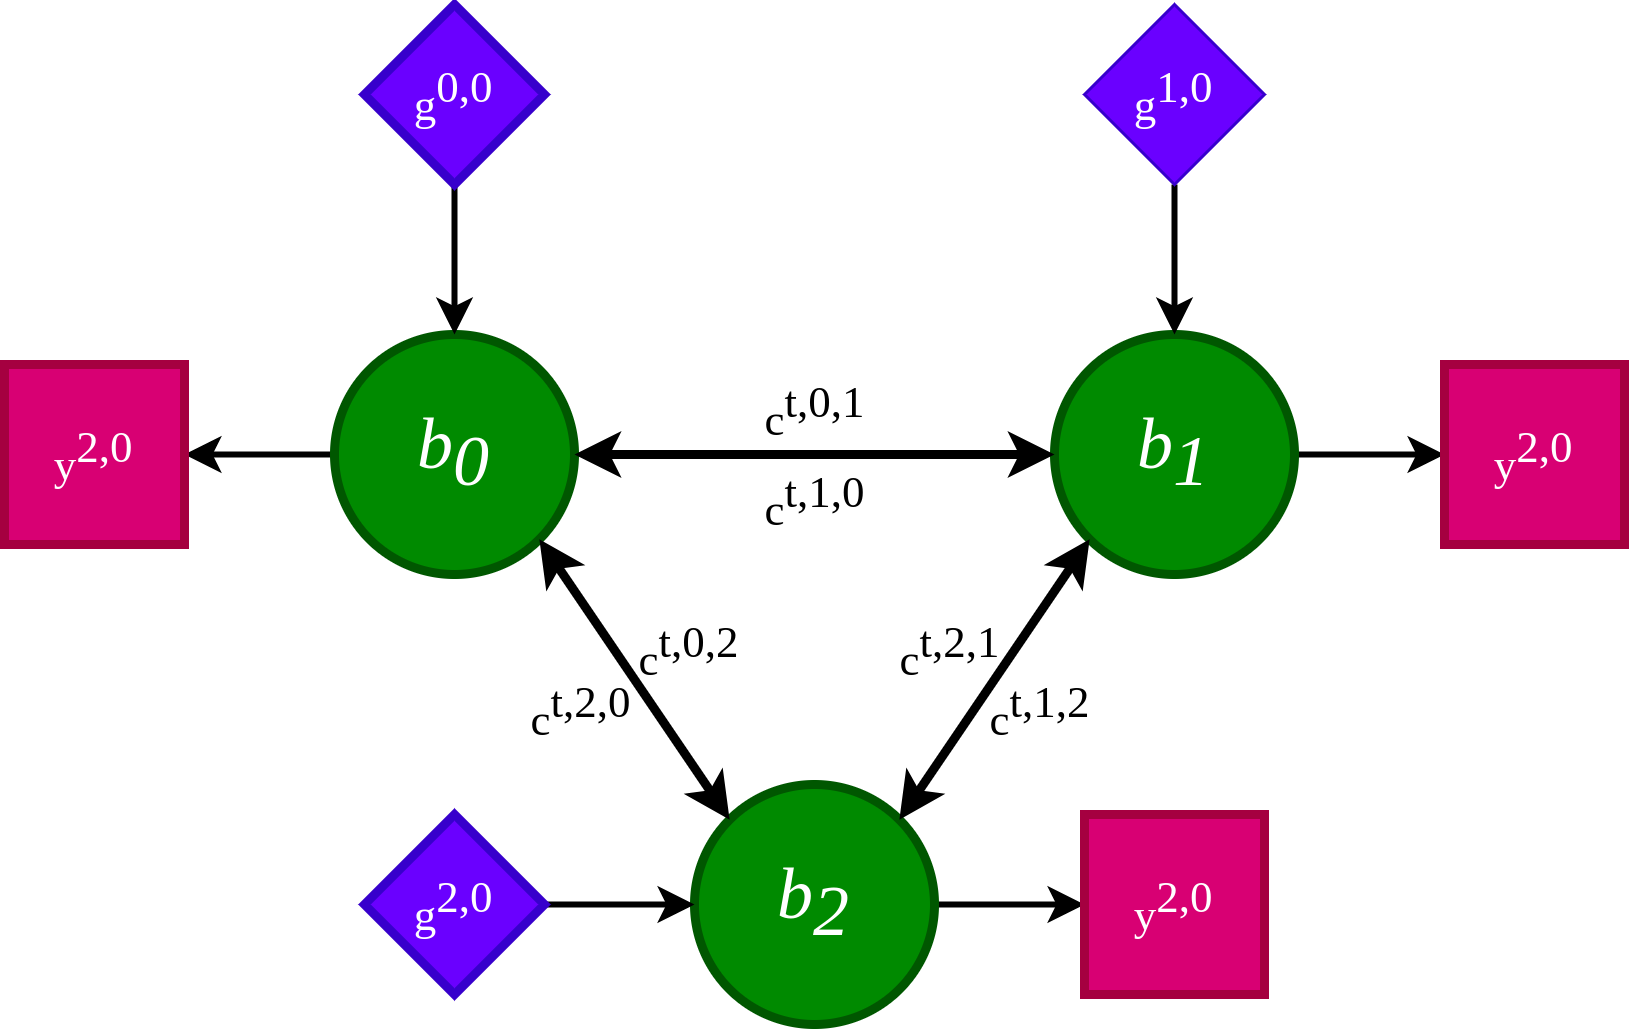
\includegraphics[width=\linewidth*2/3]{figs/3_bus_0.png}
	\caption{Simple 3 Bus Example}
	\label{fig:3_bus_0}
\end{figure}

All three buses in the example have one generator ($g$), one load ($y$), and transmission connections to the other buses. All transmission connections are bidirectional and have flow limits. Two scenarios are shown in Figure \ref{fig:3_bus_scenarios}.




 








\end{document}